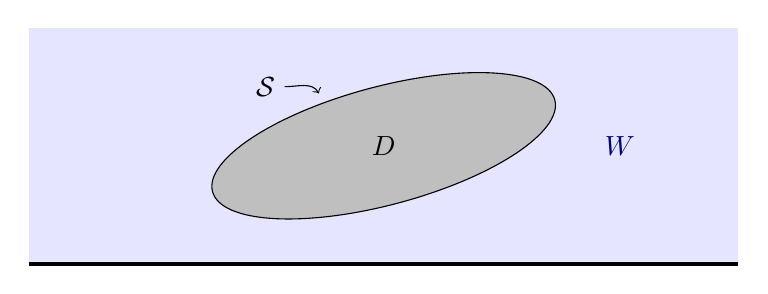
\begin{tikzpicture}[scale=1.5]
  \fill[blue!10] (-3, 0) rectangle (3, 2);
  \draw[very thick] (-3, 0) -- (3, 0);
  \draw[fill=lightgray] (0, 1) circle [x radius=1.5, y radius=.5, rotate=15];
  
  \node[blue!50!black] at (2, 1) {$W$};
  \node at (0, 1) {$D$};
  \node (label) at (-1, 1.5) {$\mathcal{S}$};
  \node (boundary) at (-.5, 1.36) {};
  \draw[->] (label) to [out=0, in=120] (boundary);
\end{tikzpicture}
